\documentclass[conference]{IEEEtran}
\usepackage{cite}
\usepackage{amsmath,amssymb,amsfonts}
\usepackage{algorithmic}
\usepackage{graphicx}
\usepackage{textcomp}
\usepackage{xcolor}
\def\BibTeX{{\rm B\kern-.05em{\sc i\kern-.025em b}\kern-.08em
    T\kern-.1667em\lower.7ex\hbox{E}\kern-.125emX}}
\begin{document}

\title{Assignment 2\\
\thanks{Identify applicable funding agency here. If none, delete this.}
}

\author{\IEEEauthorblockN{Taten H. Knight}
\IEEEauthorblockA{\textit{College of Aviation, Science and Technology} \\
\textit{Lewis University}\\
Romeoville, USA \\
knight.taten@gmail.com}
}

\maketitle

\begin{abstract}
This paper is a literature review of \emph{Comparison of Model Checking Tools}[1] and \emph{Introduction to Embedded Software Verification}[2]. It explores the contributions of each paper to the study of model checking --- one of various formal software verification methods. The papers above explore the application of model checking to Embedded Systems and Information Systems (IS). I examine the novel ideas and methods presented, the tools used, the areas of application relevant to the given information and methods, and the current and potential applications of the research to my own professional activities.
\end{abstract}

\begin{IEEEkeywords}
component, formatting, style, styling, insert
\end{IEEEkeywords}

\section{Introduction}
Formal verification is the process of verifying a software system by exploring the state-space of the system and confirming that it meets a set of specifications for all of the states. Model checking is a method of formal verification wherein a model checking software creates a model of the original software that allows it to be explored and verified using a formal logic language (CTL, LTL) [1][2]. Formal software verification methods are more pertinent as the size and complexity of software systems continues to grow and maintaining sufficient test coverage across the software is infeasible. At this point (2022) many major manufacturers such as Dassault-Aviation and Airbus are using formal verification on safety and system critical systems [3], however, at the time of the articles being written formal verification had not been widely implented in industry.

\section{Comparison of Model Checking Tools for Information Systems}

\subsection{Article Introduction}
The focus of this paper was the analysis of the performance of six model checking tools on a single case study. Performance was measured based on ease of specifying the information system (IS) properties and behavior, and on the number of IS instances that can be checked. 

\subsection{Areas of Application}
This article focuses on the use of model checking for a simple IS. An IS is the software and hardware system that supports a data-intensive application. The IS used for this case study was an extremely small-scale model of a typlical IS, a library system. A diagram of the system is shown in Fig. 1.

\begin{figure}[htbp]
\centerline{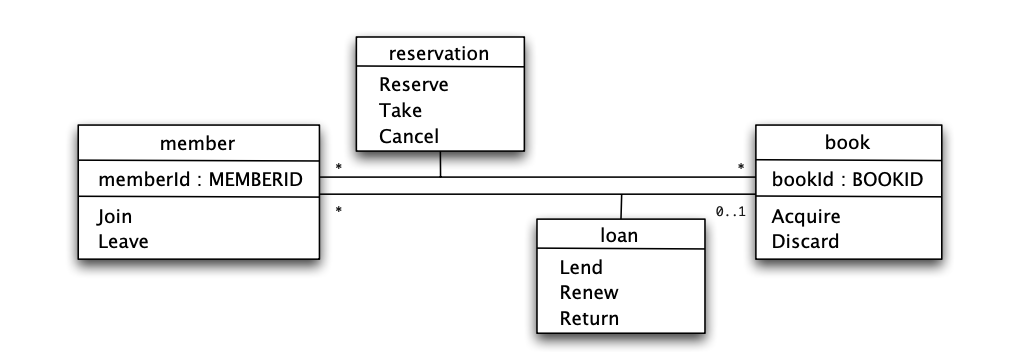
\includegraphics[width=0.5\textwidth]{./images/case_study.png}}
\caption{Requirement class diagram of the library system [1]}
\label{fig}
\end{figure}

The diagram describes the properties of the IS, for example the library has the ability to acquire any book that is not currently checked out. This and the other properties are the logic statements that can be subsequently expressed and verified through the model checker.

\subsection{Tools}
The authors and researchers focused on the comparison of six tools for model-checking:
\begin{enumerate}

\item Spin - One of the first model checkers developed. It introduced the classical approach for on-the-fly Linear Temportal Logic (LTL) model checking. It uses propositional LTL with the \emph{always}, \emph{eventually}, and \emph{until} operators. Spin has no concept of events, and a run consists of a trace with the states visited during execution.

\item NuSMV - The first implementation of Symbolic Model Checking, which uses a symbolic representation of the software to check against the specifications. It is able to deal with Computational Tree Logic (CTL), LTL, and SAT-based bounded model checking. It uses the Promela language, which is very low-level, and can result in it taking longer to write specifications. It can also be either state or event oriented, which gives flexibility.

\item fdr2 - A state model checker for Communicating Concurrent Processes (CSP). It "can check refinement, deadlocks, livelocks, and determinancy of process expressions. It builds and then compresses the state-space transition graph, which makes it an implicit model checker.

\item cadp - Uses the LOTOS NT language to specify models and XTL to specify properties. It does not naturally support state variables which can make model checking difficult.

\item Alloy - Alloy is another symbolic model checker. All properties and specifications are expressed as first-order formulae.

\item ProB - A very flexible model checker that uses the B method. "Properties in ProB can be written in LTL, past LTL or CTL, hence combining the strengths of each language." It allows for "the inclusion of first-order formulae in temporal formulae.

\end{enumerate}

\subsection{New Concepts and Knowledge}
I believe that the conclusion of the case study provided the most insight into model checker viability. A good model checker needs to be able to handle both state and events. Pure LTL is useful, but cannot be the sole language used. A pure first-order logic like Alloy can be used but may not be the most intuitive. ProB is the most 'polyvalent' model checker, meaning that it handles the most situations with model checking. The other useful information from this paper is available in the appendices. The authors provided the setup code for each of the models in the study. Fig. 2 shows the first page of code for creating the Spin model.

\begin{figure}[htbp]
\centerline{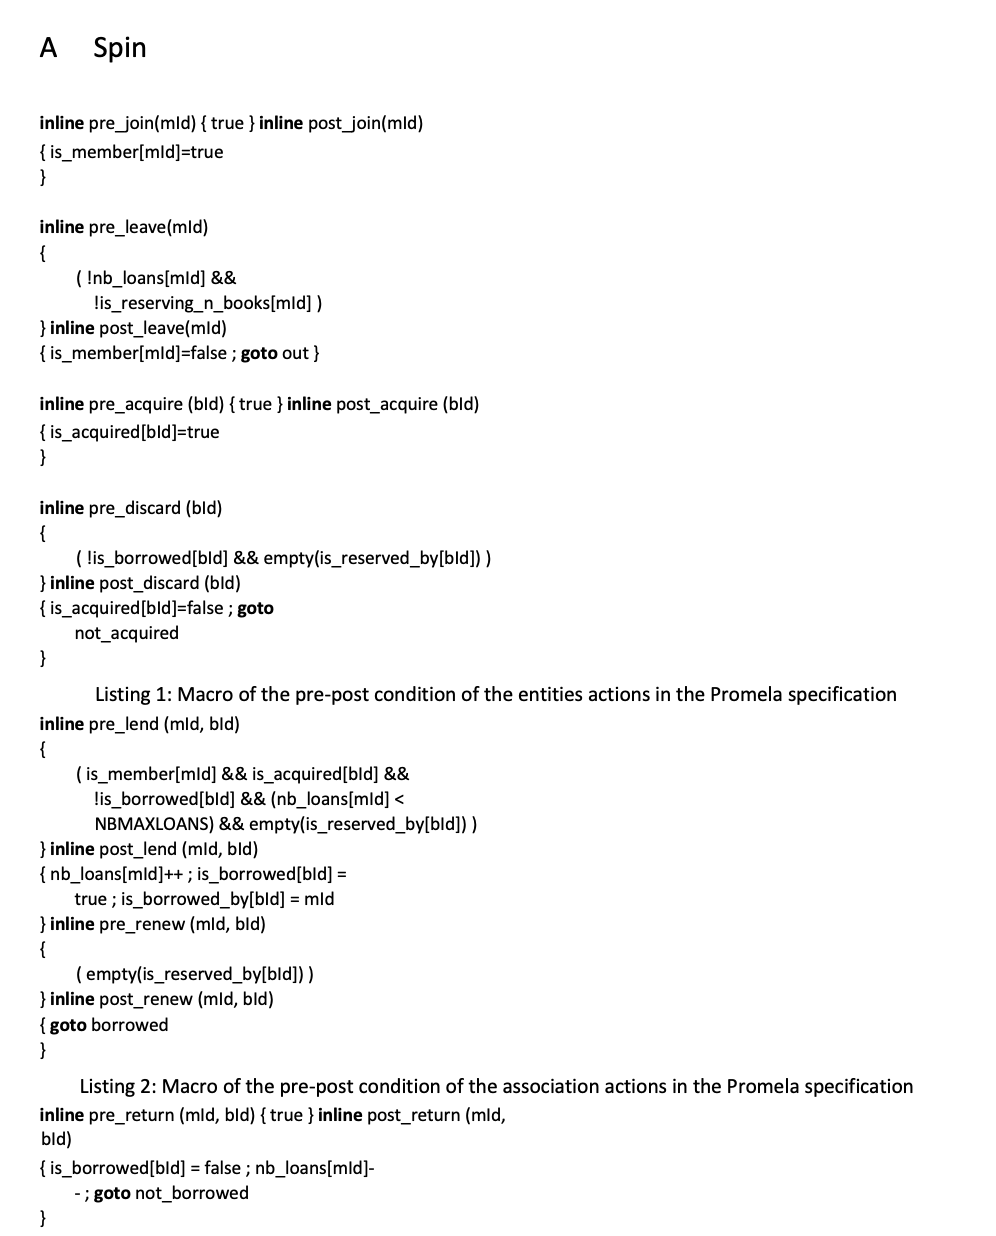
\includegraphics[width=0.5\textwidth]{./images/spin_appendix.png}}
\caption{Model specification appendix [1]}
\label{fig}
\end{figure}

Each model is a multi-page ordeal, and having reference to some of the base syntax and working example code provides a solid jumping off point for further exploration.

\subsection{Professional Applicability}
In my current professional career as a full-stack developer, the above methods are useful for potentially testing backend infrastructure and verifying that data integrity is maintained through backups, updates, deletes, or other forms of manipulations. The authors note that user interaction (including queries) are not covered in this study, so these specific methods may not be applicable for the frontend to backend to frontend flow of the full software stack.

\section{Introduction to Embedded Software Verification}

\subsection{Article Introduction}
\emph{Introduction to Embedded Software Verification} is a solid introduction to software verification in general. It covers the core concept of software verification and two of its subsets; model checking and theorem proving. It also provides an overview of how one would approach model checking on a microcontroller.

\subsection{Areas of Application}
Because this paper provides an introduction to the general concept of software verification, it can provide a precursory look into the concepts before diving into more in-depth research and literature. I would argue that because of this, the paper is widely applicable to the field as an introduction. It also covers the concept of CTL, which is used in a few of the tools mentioned in [1]. I plan on using it as a reference for reviewing easy concepts before moving onto others research. 

\subsection{Tools}
The paper is a conceptual overview and not a research paper, so there are no technical tools used. That being said, the paper does utilize some notable pedagogical tools, namely repetition and summarization to re-emphasize and solidify key points. It also shallowly explores the broader field of embedded software verification through model checking assembly code. This is a preferred technique for embedded software because once the model checker is developed for a microcontroller or similar system, it can be reused across any software that is installed on that system.

\subsection{New Concepts and Knowledge}
Using assembly code model checkers for microcontrollers and similar subsystems is and will continue to prove a valuable and useful concept for any and all large scale custom silicon and controller manufacturers. "...[V]erification effort of nowadays embedded systems projects consumes up to 70 percent of the entire engineering budget" "unpublished" [2]. Anything to reduce average overhead on development and verification of software is going to rightfully result in extreme savings.

\subsection{Professional Applicability}
Assembly level verification borders on the realm between computer science and computer engineering in my mind, and my current role doesn't sit on this border. I am, however, focusing on AI/ML in my studies, and the field as a whole is and will likely continue to move into custom silicon for AI/ML workloads. These chips will need to be verified as individual components and as part of the hardware/software stack that they are being included in. As these applications grow, having a combination of verification methods for these chips will be a necessity.

Looking even further to the future, verification of massive software systems may be made even easier with the eventual advent of quantum computing systems.

\section{Conclusion}
The two papers reviewed developed the overarching themes of software verification. \emph{Comparison of Model Checking Tools} focused on the applying model checking to IS systems, and provided an analysis of various IS model checking tools and the merits of each. It also provided detailed code in the appendices for model setup. \emph{Introduction to Embedded Software Verification} was a far simpler introductory paper to software verification as a whole. It explained the basics of software verification, theorem proving, model checking, CTL syntax, and the use of model checking on microcontroller assembly code. It is the most easily understandable reference guide to simple software verification concepts that I have found thus far. Both papers provide references and ideas that will be useful in the use of model checkers for embedded software and IS software verification, and they explore the foundations of a field that will only grow with increases in custom silicon requirements.


\begin{thebibliography}{00}
\bibitem{b1} M. Frappier, B. Fraikin, R. Chossart, R. Chane-Yack-Fa, and M. Ouenzar, ``Comparison of Model Checking Tools for Information Systems,'' International Conference on Formal Engineering Methods. Springer, Berlin, Heidelberg, 2010.
\bibitem{b2} T. Reinbacher, ''Introduction to Embedded Software Verification,'' unpublished
\bibitem{b3} Y. Moy, E. Ledinot, H. Delseny, V. Wiels and B. Monate, "Testing or Formal Verification: DO-178C Alternatives and Industrial Experience" in IEEE Software, vol. 30, no. 03, pp. 50-57, 2013.
\end{thebibliography}

\end{document}
